\tikzset{every picture/.style={line width=0.75pt}} %set default line width to 0.75pt        

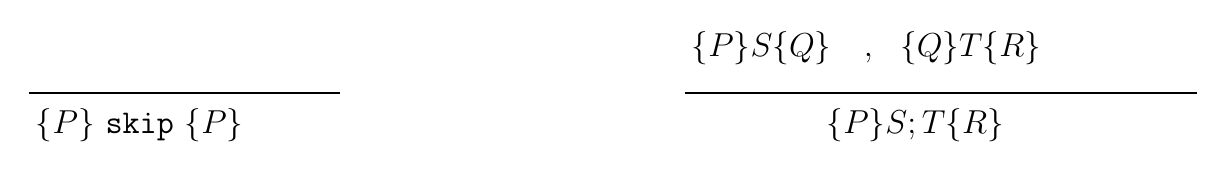
\begin{tikzpicture}[x=0.75pt,y=0.75pt,yscale=-1,xscale=1]
%uncomment if require: \path (0,104); %set diagram left start at 0, and has height of 104

%Straight Lines [id:da43085718847463716] 
\draw    (92,53) -- (242,53) ;
%Straight Lines [id:da073972515186154] 
\draw    (408,53) -- (655,53) ;

% Text Node
\draw (410,22) node [anchor=north west][inner sep=0.75pt]  [font=\large]  {$\{P\} S\{Q\} \ \ \ ,\ \ \{Q\} T\{R\}$};
% Text Node
\draw (94, 59) node [anchor=north west][inner sep=0.75pt]  [font=\large]  {$\{P\} \ \mathtt{skip} \ \{P\}$};
% Text Node
\draw (475,59) node [anchor=north west][inner sep=0.75pt]  [font=\large]  {$\{P\} S;T\{R\}$};


\end{tikzpicture}
